\documentclass[10pt, conference]{IEEEtran}
\usepackage[english]{babel}
\usepackage[T1]{fontenc}
\usepackage[usenames]{color}
\usepackage{colortbl}
\usepackage{comment}
\usepackage{graphicx}
\usepackage{array, colortbl}
\usepackage{multirow}
\usepackage{booktabs}
\usepackage{float}
\usepackage[obeyspaces,hyphens,spaces]{url}
\usepackage{balance}
\usepackage[normalem]{ulem}
\usepackage{xspace}
\usepackage{microtype}
\usepackage{pgfgantt}
\usetikzlibrary{arrows.meta, positioning}
\usepackage{listings}
\lstset{basicstyle=\ttfamily\scriptsize, breaklines=true, columns=fullflexible,
  frame=single, framerule=0.4pt, xleftmargin=2pt, xrightmargin=2pt, showstringspaces=false}
\pagenumbering{arabic}
\pagestyle{empty}
\clubpenalty = 10000
\widowpenalty = 10000
\displaywidowpenalty = 10000
\usepackage{cleveref}
\crefname{figure}{Fig.}{Figs.}

\makeatletter
\renewcommand{\paragraph}[1]{\noindent\textbf{#1}.}
\makeatother

% Every number below is a macro generated from results/numbers.json by src/make_macros.py.
% Generated by src/make_macros.py from results/numbers.json. Do not edit by hand.
\newcommand{\ciFossil}{[19.3, 19.9]\%\xspace}
\newcommand{\ciNeverRevised}{[62.4, 63.1]\%\xspace}
\newcommand{\ciPlaceholder}{[28.9, 29.6]\%\xspace}
\newcommand{\numArchivePlaceholder}{19{,}651\xspace}
\newcommand{\numArchived}{156{,}372\xspace}
\newcommand{\numCohortCommits}{735{,}667\xspace}
\newcommand{\numCohortSpecs}{468{,}163\xspace}
\newcommand{\numCommitTable}{780{,}335\xspace}
\newcommand{\numDelta}{41{,}582\xspace}
\newcommand{\numDroppedSpecs}{2{,}632\xspace}
\newcommand{\numFlagOnly}{1{,}674\xspace}
\newcommand{\numFossilRepos}{2{,}488\xspace}
\newcommand{\numFossils}{14{,}294\xspace}
\newcommand{\numFossilsArchiveText}{13{,}426\xspace}
\newcommand{\numLiving}{72{,}971\xspace}
\newcommand{\numLivingOldNinety}{26{,}887\xspace}
\newcommand{\numLivingRepos}{6{,}085\xspace}
\newcommand{\numLivingYoungThirty}{16{,}099\xspace}
\newcommand{\numNoBoth}{1{,}329\xspace}
\newcommand{\numNoContent}{2{,}488\xspace}
\newcommand{\numNoHistory}{1{,}473\xspace}
\newcommand{\numOpenSpecFiles}{274{,}955\xspace}
\newcommand{\numOpenSpecRepos}{8{,}926\xspace}
\newcommand{\numOrphanCommits}{41{,}170\xspace}
\newcommand{\numPlaceholderRevised}{7{,}031\xspace}
\newcommand{\numRenameChecked}{30\xspace}
\newcommand{\numRenameLivingChecked}{15\xspace}
\newcommand{\numRenameLivingTrue}{1\xspace}
\newcommand{\numRenamePlainMatch}{29\xspace}
\newcommand{\numRepoK}{3\xspace}
\newcommand{\numRepos}{73{,}030\xspace}
\newcommand{\numReposK}{4{,}618\xspace}
\newcommand{\numRevised}{27{,}184\xspace}
\newcommand{\numSampleFossils}{375\xspace}
\newcommand{\numSampleFossilsTen}{96\xspace}
\newcommand{\numSampleRevised}{379\xspace}
\newcommand{\numSampleRevisedTen}{96\xspace}
\newcommand{\numSpecFiles}{470{,}795\xspace}
\newcommand{\pctArchivedNeverRevised}{96.7\%\xspace}
\newcommand{\pctConfSample}{95\%\xspace}
\newcommand{\pctDeltaNeverRevised}{89.7\%\xspace}
\newcommand{\pctFlagPrecision}{92.2\%\xspace}
\newcommand{\pctFlagPurposeTbd}{98.7\%\xspace}
\newcommand{\pctFlagRecall}{100.0\%\xspace}
\newcommand{\pctFossil}{19.6\%\xspace}
\newcommand{\pctFossilOldNinety}{16.8\%\xspace}
\newcommand{\pctLivingYoungNinety}{63\%\xspace}
\newcommand{\pctLivingYoungThirty}{22\%\xspace}
\newcommand{\pctNeverRevised}{62.7\%\xspace}
\newcommand{\pctNeverRevisedOldNinety}{58.0\%\xspace}
\newcommand{\pctNoPlaceholder}{70.8\%\xspace}
\newcommand{\pctOpenSpecFiles}{58.4\%\xspace}
\newcommand{\pctPlaceholder}{29.2\%\xspace}
\newcommand{\pctPlaceholderRevised}{9.6\%\xspace}
\newcommand{\pctReposAllFossil}{7\%\xspace}
\newcommand{\pctReposExtreme}{70\%\xspace}
\newcommand{\pctReposZeroFossil}{56\%\xspace}
\newcommand{\pctTopFossilRepo}{0.94\%\xspace}

\newcommand{\fp}[1]{\texttt{#1}}

\title{The Myth of the ``Living'' Document:\\Are OpenSpec's Living Specifications Ever Revised?}
% TODO(team): add e-mail addresses.
\author{\IEEEauthorblockN{Tran Vo \quad Thanh Nghiep Quan}
\IEEEauthorblockA{\emph{Dep. of Computer and Software Engineering, Polytechnique Montr\'eal}, Montr\'eal, Canada}}

\begin{document}
\maketitle

\begin{abstract}
In spec-driven development (SDD), developers describe what to build in a Markdown
specification and an AI coding agent implements it. OpenSpec, the SDD tool with the most
spec files in SpecMine (the MSR 2027 Mining Challenge dataset), keeps one \emph{living} spec
per capability and calls it the source of truth.
We ask whether living specs are actually maintained. In a preliminary analysis of
\numLiving living specs, \pctNeverRevised were never revised after creation, and
\pctFossil (\numFossils specs) are \emph{fossils}: they still hold a TBD placeholder in
their Purpose section, usually the one OpenSpec's archive step writes, and nobody ever
edited them.
We pose four research questions: how many living specs get revised or become fossils,
what characterizes each group, and how the two differ.
\end{abstract}

\section{Problem Statement}
\label{sec:statement}

SDD tools such as OpenSpec~\cite{openspec} and GitHub Spec Kit~\cite{speckit} make the
specification the input of AI coding agents~\cite{boeckeler2025}. A \emph{spec} is a
Markdown file, written before or alongside the code, that describes what a system should
do. In OpenSpec, a developer
proposes a change (\fp{changes/<name>/} with a proposal, delta specs, a design and tasks),
the agent implements it, and \emph{archiving} moves the change to \fp{changes/archive/}
and merges its delta specs into \fp{openspec/specs/} (\cref{fig:workflow}). The specs there are \emph{living
specs}: each describes how one capability of the system currently behaves and is meant to
be updated whenever an archived change affects that capability. OpenSpec calls them the
source of truth~\cite{openspec}, and agents read them before every later change. A spec
that stops changing while the code moves on is wrong input for the next agent.

OpenSpec gives us an unusual marker of unfinished documentation. Before v1.7.0, archiving a
change that introduced a new capability always wrote
``\texttt{TBD - created by archiving change <name>. Update Purpose after archive.}'' into the
new spec's Purpose section~\cite{openspec_pr1431}. The fix (PR~\#1431) shipped on
July 29, 2026, after SpecMine's crawl ended (July 11), so any spec in the snapshot could
have received the placeholder. A spec that still holds it and was never revised was written
once and never finished (\cref{fig:example}); it is also stale only if its code moved on (RQ3).

Outdated documentation is a long-standing problem~\cite{lethbridge2003,aghajani2019,tan2024}.
The SpecMine authors list spec lifecycle, including ``placeholders never filled,'' as an
open question~\cite{specmine_paper}. Their practitioners report \emph{spec decay}, which
commit counts alone cannot show~\cite{specmine_paper}; we add a tool-written marker.

\paragraph{Link with the course} Living specs are configuration for AI agents, kept as
code; their staleness mirrors configuration drift. OpenSpec has since added a validation
check for the placeholder~\cite{openspec_pr1671}, a gate a CI pipeline can enforce; we
measure how often such a gate would fire on existing specs.

\begin{figure*}[t]
\centering
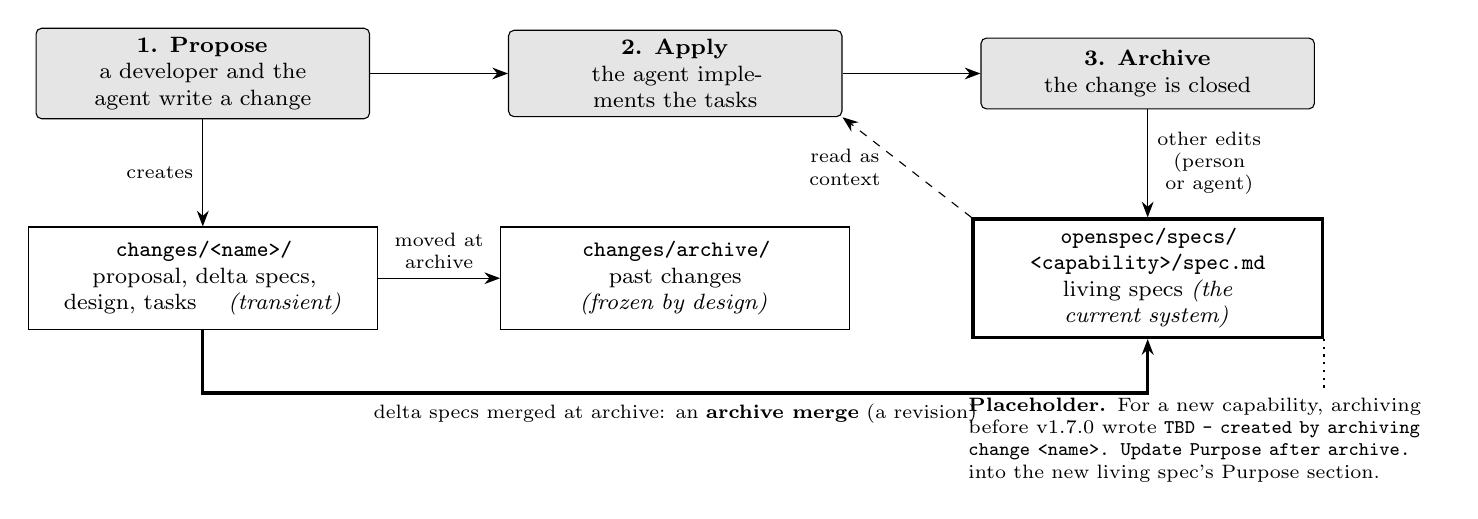
\begin{tikzpicture}[font=\footnotesize, >={Stealth[length=2mm]},
  stage/.style={draw, rounded corners=2pt, fill=black!10, align=center, text width=40mm,
    minimum height=9mm},
  folder/.style={draw, align=center, text width=42mm, minimum height=13mm},
  lab/.style={font=\scriptsize, align=center},
  note/.style={align=left, font=\scriptsize, text width=60mm}]
\node[stage] (P) at (0,0) {\textbf{1. Propose}\\a developer and the agent write a change};
\node[stage] (A) at (6,0) {\textbf{2. Apply}\\the agent implements the tasks};
\node[stage] (R) at (12,0) {\textbf{3. Archive}\\the change is closed};
\draw[->] (P) -- (A); \draw[->] (A) -- (R);
\node[folder] (C) at (0,-2.6) {\fp{changes/<name>/}\\proposal, delta specs,\\design, tasks
  \quad\emph{(transient)}};
\node[folder] (H) at (6,-2.6) {\fp{changes/archive/}\\past changes\\\emph{(frozen by design)}};
\node[folder, very thick] (S) at (12,-2.6) {\fp{openspec/specs/}\\\fp{<capability>/spec.md}\\
  living specs \emph{(the current system)}};
\draw[->] (P) -- node[lab, left] {creates} (C);
\draw[->, dashed] (S.north west) -- node[lab, left=6pt, pos=0.5] {read as\\context} (A.south east);
\draw[->] (C) -- node[lab, above] {moved at\\archive} (H);
\draw[->, very thick] (C.south) -- ++(0,-0.8) -| node[pos=0.25, below, lab]
  {delta specs merged at archive: an \textbf{archive merge} (a revision)} (S.south);
\draw[->] (R.south) -- node[lab, right] {other edits\\(person\\or agent)} (S.north);
\node[note, anchor=north west] (N) at (9.6,-4.0) {\textbf{Placeholder.} For a new capability,
  archiving before v1.7.0 wrote \fp{TBD - created by archiving change <name>. Update Purpose
  after archive.} into the new living spec's Purpose section.};
\draw[dotted, thick] (S.south east) -- (S.south east |- N.north);
\end{tikzpicture}
\caption{The OpenSpec workflow and the three folders. A revision of a living spec is either an
archive merge or another edit; a fossil is a living spec that still holds the placeholder and
has no revision.}
\label{fig:workflow}
\end{figure*}

\begin{figure}[t]
\lstinputlisting{../results/example_fossil_spec.md}
\caption{A fossil from SpecMine: the Purpose still holds the archive placeholder, while the
requirements are complete. The spec was chosen at random with a fixed seed by
\fp{src/s05\_example\_fossil.py}. Lightly edited: the repository, the change name, paths and
package names are masked.}
\label{fig:example}
\end{figure}

\section{Research Questions}
\label{sec:research-idea}

All analyses start from \emph{commits per spec file}. A \emph{revision} is a
commit that touches the file after its creation commit. We separate
\emph{archive merges}, the revisions written by OpenSpec's archive step (commits that also create a file under
\fp{changes/archive/}), from other edits. An archive merge follows automatically from
archiving a change, so it says little about whether anyone chose to maintain the spec;
other edits are deliberate. A
\emph{fossil} is a living spec whose snapshot content holds an unfilled placeholder and
that has zero revisions.

\textbf{RQ1: What portion of living specs get revised, and how many become fossils?}
\emph{Motivation:} if living specs are the source of truth, each archived change that
touches a capability should revise its spec; the naive ``never revised'' rate mixes
finished specs with forgotten ones, and the placeholder helps tell them apart.
\emph{Approach:} revisions per living spec, split into archive merges and other edits; the
shares of fossils, of specs whose placeholder survived a revision and of specs without one,
among all living specs and among specs born with the placeholder (to be decided); Wilson
95\% CIs (or a bootstrap over repositories: to be decided).
\emph{Baselines:} archived specs, frozen by design (\pctArchivedNeverRevised never
revised), and delta specs; the naive measure; a no-placeholder control group.
\emph{Robustness:} file age: \pctLivingYoungThirty of living specs are under 30 days old,
so we re-run every result without specs younger than 30, 60 and 90 days (for specs at
least 90 days old, \pctNeverRevisedOldNinety were never revised and \pctFossilOldNinety are
fossils); repository dominance: per-repository caps and leave-largest-out.

\textbf{RQ2: What characterizes living specs that are revised?} \emph{Motivation:}
revised specs show what maintenance looks like in practice.
\emph{Approach:} the time to first revision (Kaplan--Meier, censored at the
snapshot), who revised (human, agent or bot), whether each revision was an archive
merge or another edit and, on the sample, the spec category (both defined below). For \emph{fixed} specs (first
version with the placeholder, snapshot without; found with \texttt{git log -p} on cloned
repositories), we record who filled the placeholder.
\emph{Baseline:} counting archive merges as maintenance.

\textbf{RQ3: What characterizes fossils?} \emph{Motivation:} a fossil may be a finished
spec whose Purpose nobody filled or a forgotten one whose code moved on.
\emph{Approach:} repository activity after creation, bulk creation (other specs
created in the same commit) and, on the sample, the spec category, completeness and
whether the code the spec describes changed later. \emph{Baselines:} never-revised specs
without a placeholder; inactive repositories separate forgotten from finished specs.

\textbf{RQ4: How do revised living specs and fossils differ?} \emph{Motivation:}
the contrast shows which traits go with maintenance. \emph{Approach:} we compare
the two groups on the features of RQ2--RQ3 with $\chi^2$ tests and Cram\'er's~$V$, and
report never-revised specs without a placeholder as a third group (to be decided). \emph{Baseline:} the
naive split into never-revised and revised specs.

\paragraph{Sampling and coding} Per repository, we sample at most one fossil and one
revised spec, with a fixed seed: about \numSampleFossils fossils and \numSampleRevised
revised specs (\pctConfSample confidence, $\pm$5\%). \emph{Spec category:} we reuse
the taxonomy and judge prompts of SpecMine~\cite{specmine_paper}:
requirements content (problem, behaviour, acceptance, constraints, stakeholders) and
implementation content (architecture, plan, code, conventions), each with an extent from
none to dominant, and the kind of work (purpose: feat, fix, refactor, style, perf; object:
docs, test, ci, build, chore). We add our own dimension, completeness (complete
except Purpose, skeletal, near-empty). Both students code a pilot of 30 specs to check
whether the taxonomy fits living specs, which describe a system as it stands, or needs
extending, then double-code 100 (Cohen's~$\kappa$). An LLM (temperature~0, tuned
on the pilot only) labels the rest if it reaches $\kappa \geq 0.6$ on held-out human
labels. A planned extension compares tools without archived
specs, as only OpenSpec encodes lifecycle roles~\cite{specmine_paper}.

\begin{figure*}[t]
\centering
\begin{ganttchart}[time slot format=isodate, x unit=0.27cm, y unit chart=0.42cm,
  y unit title=0.42cm, hgrid, vgrid={*{6}{draw=none}, dotted},
  title label font=\tiny, bar label font=\footnotesize, milestone label font=\footnotesize,
  bar height=0.55, bar/.append style={fill=black!35, draw=black!70},
  milestone/.append style={fill=black!80, draw=black}]{2026-11-09}{2026-12-23}
\gantttitlecalendar{month=name, day} \\
\ganttbar{RQ1; samples; pilot (30 specs)}{2026-11-09}{2026-11-15} \\
\ganttbar{Double coding ($\kappa$)}{2026-11-16}{2026-11-18} \\
\ganttbar{LLM labelling; RQ2--RQ4}{2026-11-19}{2026-11-22} \\
\ganttmilestone{Numbers frozen}{2026-11-22} \\
\ganttmilestone{Presentation}{2026-11-26} \\
\ganttmilestone{Report; MSR abstract}{2026-12-18} \\
\ganttmilestone{MSR paper}{2026-12-23}
\end{ganttchart}
\caption{Plan from November 9, 2026 (dotted lines separate weeks, Monday to Sunday).}
\label{fig:gantt}
\end{figure*}

\section{Dataset}
\label{sec:dataset}
\sloppy

We use SpecMine v1.0 (July 2026 snapshot)~\cite{specmine_dataset,specmine_paper}:
\numSpecFiles spec files from \numRepos GitHub repositories. OpenSpec accounts for
\numOpenSpecFiles files (\pctOpenSpecFiles) in \numOpenSpecRepos repositories. We query the
Parquet tables with DuckDB: \texttt{spec\_files} (tool, lifecycle role),
\texttt{spec\_file\_commits} (per-file history) and \texttt{spec\_content\_features} (the
placeholder flag), plus snapshot texts (\texttt{specs.jsonl.gz}, Zenodo only). Our cohort
keeps the \numCohortSpecs specs with both a fetched commit history and fetched content
(\numCohortCommits commits); the \numDroppedSpecs excluded files lack history
(\numNoHistory) or content (\numNoContent); \numNoBoth of them lack both.
\Cref{tab:prelim} gives our preliminary numbers. \Cref{fig:repo} shows that fossils
cluster by repository: \pctReposExtreme of repositories with at least \numRepoK living
specs have a fossil rate at or below 10\% or at or above 90\%, so we sample fossils per
repository.

\begin{figure}[t]
\centering
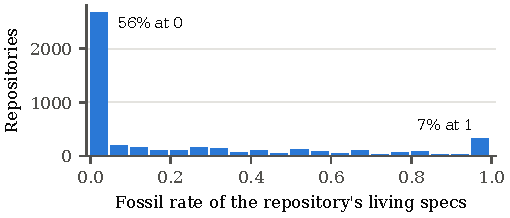
\includegraphics[width=0.9\columnwidth]{../results/figures/repo_fossil_rate.pdf}
\caption{Fossil rate per repository ($\geq$\numRepoK living specs; \numReposK repositories).}
\label{fig:repo}
\end{figure}

\begin{table}[t]
\centering
\caption{Preliminary results for OpenSpec living specs (Wilson CIs)}
\label{tab:prelim}
\footnotesize
\begin{tabular}{@{}lrr@{}}
\toprule
Quantity & Value & 95\% CI \\
\midrule
Living / delta / archived specs & \multicolumn{2}{r@{}}{\numLiving\,/\,\numDelta\,/\,\numArchived} \\
Living specs never revised & \pctNeverRevised & \ciNeverRevised \\
Unfilled placeholder & \pctPlaceholder & \ciPlaceholder \\
\quad and never revised (fossil) & \pctFossil & \ciFossil \\
\quad and revised at least once & \pctPlaceholderRevised & \\
Repos with fossils (largest share: \pctTopFossilRepo) & \numFossilRepos & \\
\bottomrule
\end{tabular}
\end{table}

\paragraph{Data caveats we already checked} (1)~Histories do not follow renames: in
\numRenamePlainMatch of \numRenameChecked sampled specs, SpecMine's commit count equals a
path-only \texttt{git log}, and \numRenameLivingTrue of the \numRenameLivingChecked living
specs was renamed, so revision counts are lower bounds. (2)~The placeholder flag (snapshot
only) catches all \numArchivePlaceholder specs with the archive text; \pctFlagPrecision of
flagged specs hold that text, \pctFlagPurposeTbd some TBD Purpose.
(3)~SpecMine has no code commits outside its pull-request layer, so code activity and
fixed specs require cloning repositories.

\section{Related Work}
\label{sec:related}

\paragraph{SDD and SpecMine} Agarwal et al.~\cite{specmine_paper} release SpecMine and
study SDD through interviews and 266 repositories; they report that living specs decay but
do not measure it. We do, with per-file history over all \numLiving living specs.

\paragraph{Outdated documentation} Documentation is often out of
date~\cite{lethbridge2003}, up-to-dateness is part of documentation-issue
taxonomies~\cite{aghajani2019}, and outdated code references can be detected in READMEs
and wikis~\cite{tan2024}; we study specs the tool labels current.

\paragraph{Self-admitted technical debt} Potdar and Shihab~\cite{potdar2014} and Bavota and
Russo~\cite{bavota2016} study debt that developers admit in code comments and whether it is
removed. In our setting the tool writes the debt marker, and we ask whether anyone pays it.

\section{Time Planning of Project}
\label{sec:schedule}
\Cref{fig:gantt} shows the plan from November 9, 2026. Numbers are frozen on November 22;
the course report and the MSR 2027 Mining Challenge abstract are due on December 18, and the
challenge paper (4 pages plus references, double-blind) on December 23.


\balance
\bibliographystyle{IEEEtran}
\bibliography{proposal.bib}
\end{document}
